\documentclass[11pt, a4paper]{article}
\usepackage{pdfpages}
\usepackage{parallel}
\usepackage[T2A]{fontenc}
\usepackage{ucs}
\usepackage[utf8x]{inputenc}
\usepackage[polish,english,russian]{babel}
\usepackage{hyperref}
\usepackage{rotating}
\usepackage[inner=2cm,top=1.8cm,outer=2cm,bottom=2.3cm,nohead]{geometry}
\usepackage{listings}
\usepackage{graphicx}
\usepackage{wrapfig}
\usepackage{longtable}
\usepackage{indentfirst}
\usepackage{array}
\usepackage{tikzsymbols}
\usepackage{soul}
\usepackage[ruled,vlined]{algorithm2e}
%\counterwithout{figure}{section} 

\usepackage{url}
\makeatletter
\g@addto@macro{\UrlBreaks}{\UrlOrds}
\makeatother

\newcolumntype{P}[1]{>{\raggedright\arraybackslash}p{#1}}
\frenchspacing
\usepackage{fixltx2e} %text sub- and superscripts
\usepackage{icomma} % коскі ў матэматычным рэжыме
\PreloadUnicodePage{4}

\newcommand{\longpage}{\enlargethispage{\baselineskip}}
\newcommand{\shortpage}{\enlargethispage{-\baselineskip}}

\def\switchlang#1{\expandafter\csname switchlang#1\endcsname}
\def\switchlangbe{
\let\saverefname=\refname%
\def\refname{Літаратура}%
\def\figurename{Іл.}%
}
\def\switchlangen{
\let\saverefname=\refname%
\def\refname{References}%
\def\figurename{Fig.}%
}
\def\switchlangru{
\let\saverefname=\refname%
\let\savefigurename=\figurename%
\def\refname{Литература}%
\def\figurename{Рис.}%
}

\hyphenation{admi-ni-stra-tive}
\hyphenation{ex-pe-ri-ence}
\hyphenation{fle-xi-bi-li-ty}
\hyphenation{Py-thon}
\hyphenation{ma-the-ma-ti-cal}
\hyphenation{re-ported}
\hyphenation{imp-le-menta-tions}
\hyphenation{pro-vides}
\hyphenation{en-gi-neering}
\hyphenation{com-pa-ti-bi-li-ty}
\hyphenation{im-pos-sible}
\hyphenation{desk-top}
\hyphenation{elec-tro-nic}
\hyphenation{com-pa-ny}
\hyphenation{de-ve-lop-ment}
\hyphenation{de-ve-loping}
\hyphenation{de-ve-lop}
\hyphenation{da-ta-ba-se}
\hyphenation{plat-forms}
\hyphenation{or-ga-ni-za-tion}
\hyphenation{pro-gramming}
\hyphenation{in-stru-ments}
\hyphenation{Li-nux}
\hyphenation{sour-ce}
\hyphenation{en-vi-ron-ment}
\hyphenation{Te-le-pathy}
\hyphenation{Li-nux-ov-ka}
\hyphenation{Open-BSD}
\hyphenation{Free-BSD}
\hyphenation{men-ti-on-ed}
\hyphenation{app-li-ca-tion}

\def\progref!#1!{\texttt{#1}}
\renewcommand{\arraystretch}{2} %Іначай формулы ў матрыцы зліпаюцца з лініямі
\usepackage{array}

\def\interview #1 (#2), #3, #4, #5\par{

\section[#1, #3, #4]{#1 -- #3, #4}
\def\qname{LVEE}
\def\aname{#1}
\def\q ##1\par{{\noindent \bf \qname: ##1 }\par}
\def\a{{\noindent \bf \aname: } \def\qname{L}\def\aname{#2}}
}

\def\interview* #1 (#2), #3, #4, #5\par{

\section*{#1\\{\small\rm #3, #4. #5}}
\ifx\ParallelWhichBox\undefined%
    \addcontentsline{toc}{section}{#1, #3, #4}%
\else%
\ifnum\ParallelWhichBox=0%
    \addcontentsline{toc}{section}{#1, #3, #4}%
\fi\fi%

\def\qname{LVEE}
\def\aname{#1}
\def\q ##1\par{{\noindent \bf \qname: ##1 }\par}
\def\a{{\noindent \bf \aname: } \def\qname{L}\def\aname{#2}}
}

\newcommand{\interviewfooter}[1]{
\vskip 1em
\noindent \textit{#1}
}


\begin{document}

\title{1997 "--- Fellowes Sphere Trackball}
\date{}
\maketitle
Fellowes Sphere Trackball — типичный представитель данного типа указательных устройств ввода информации для компьютера, наиболее характерных для первой половины 90-х годов (хотя и выпущен компанией Fellowes Computerware в 1997). Поскольку трекбол аналогичен мыши по принципу действия и по функциям, но появился раньше, чем мышь, широко распространено мнение, что мышь была изобретена путем переворачивания трекбола вверх дном и его перемещения по поверхности стола.

\begin{figure}[h]
    \centering
    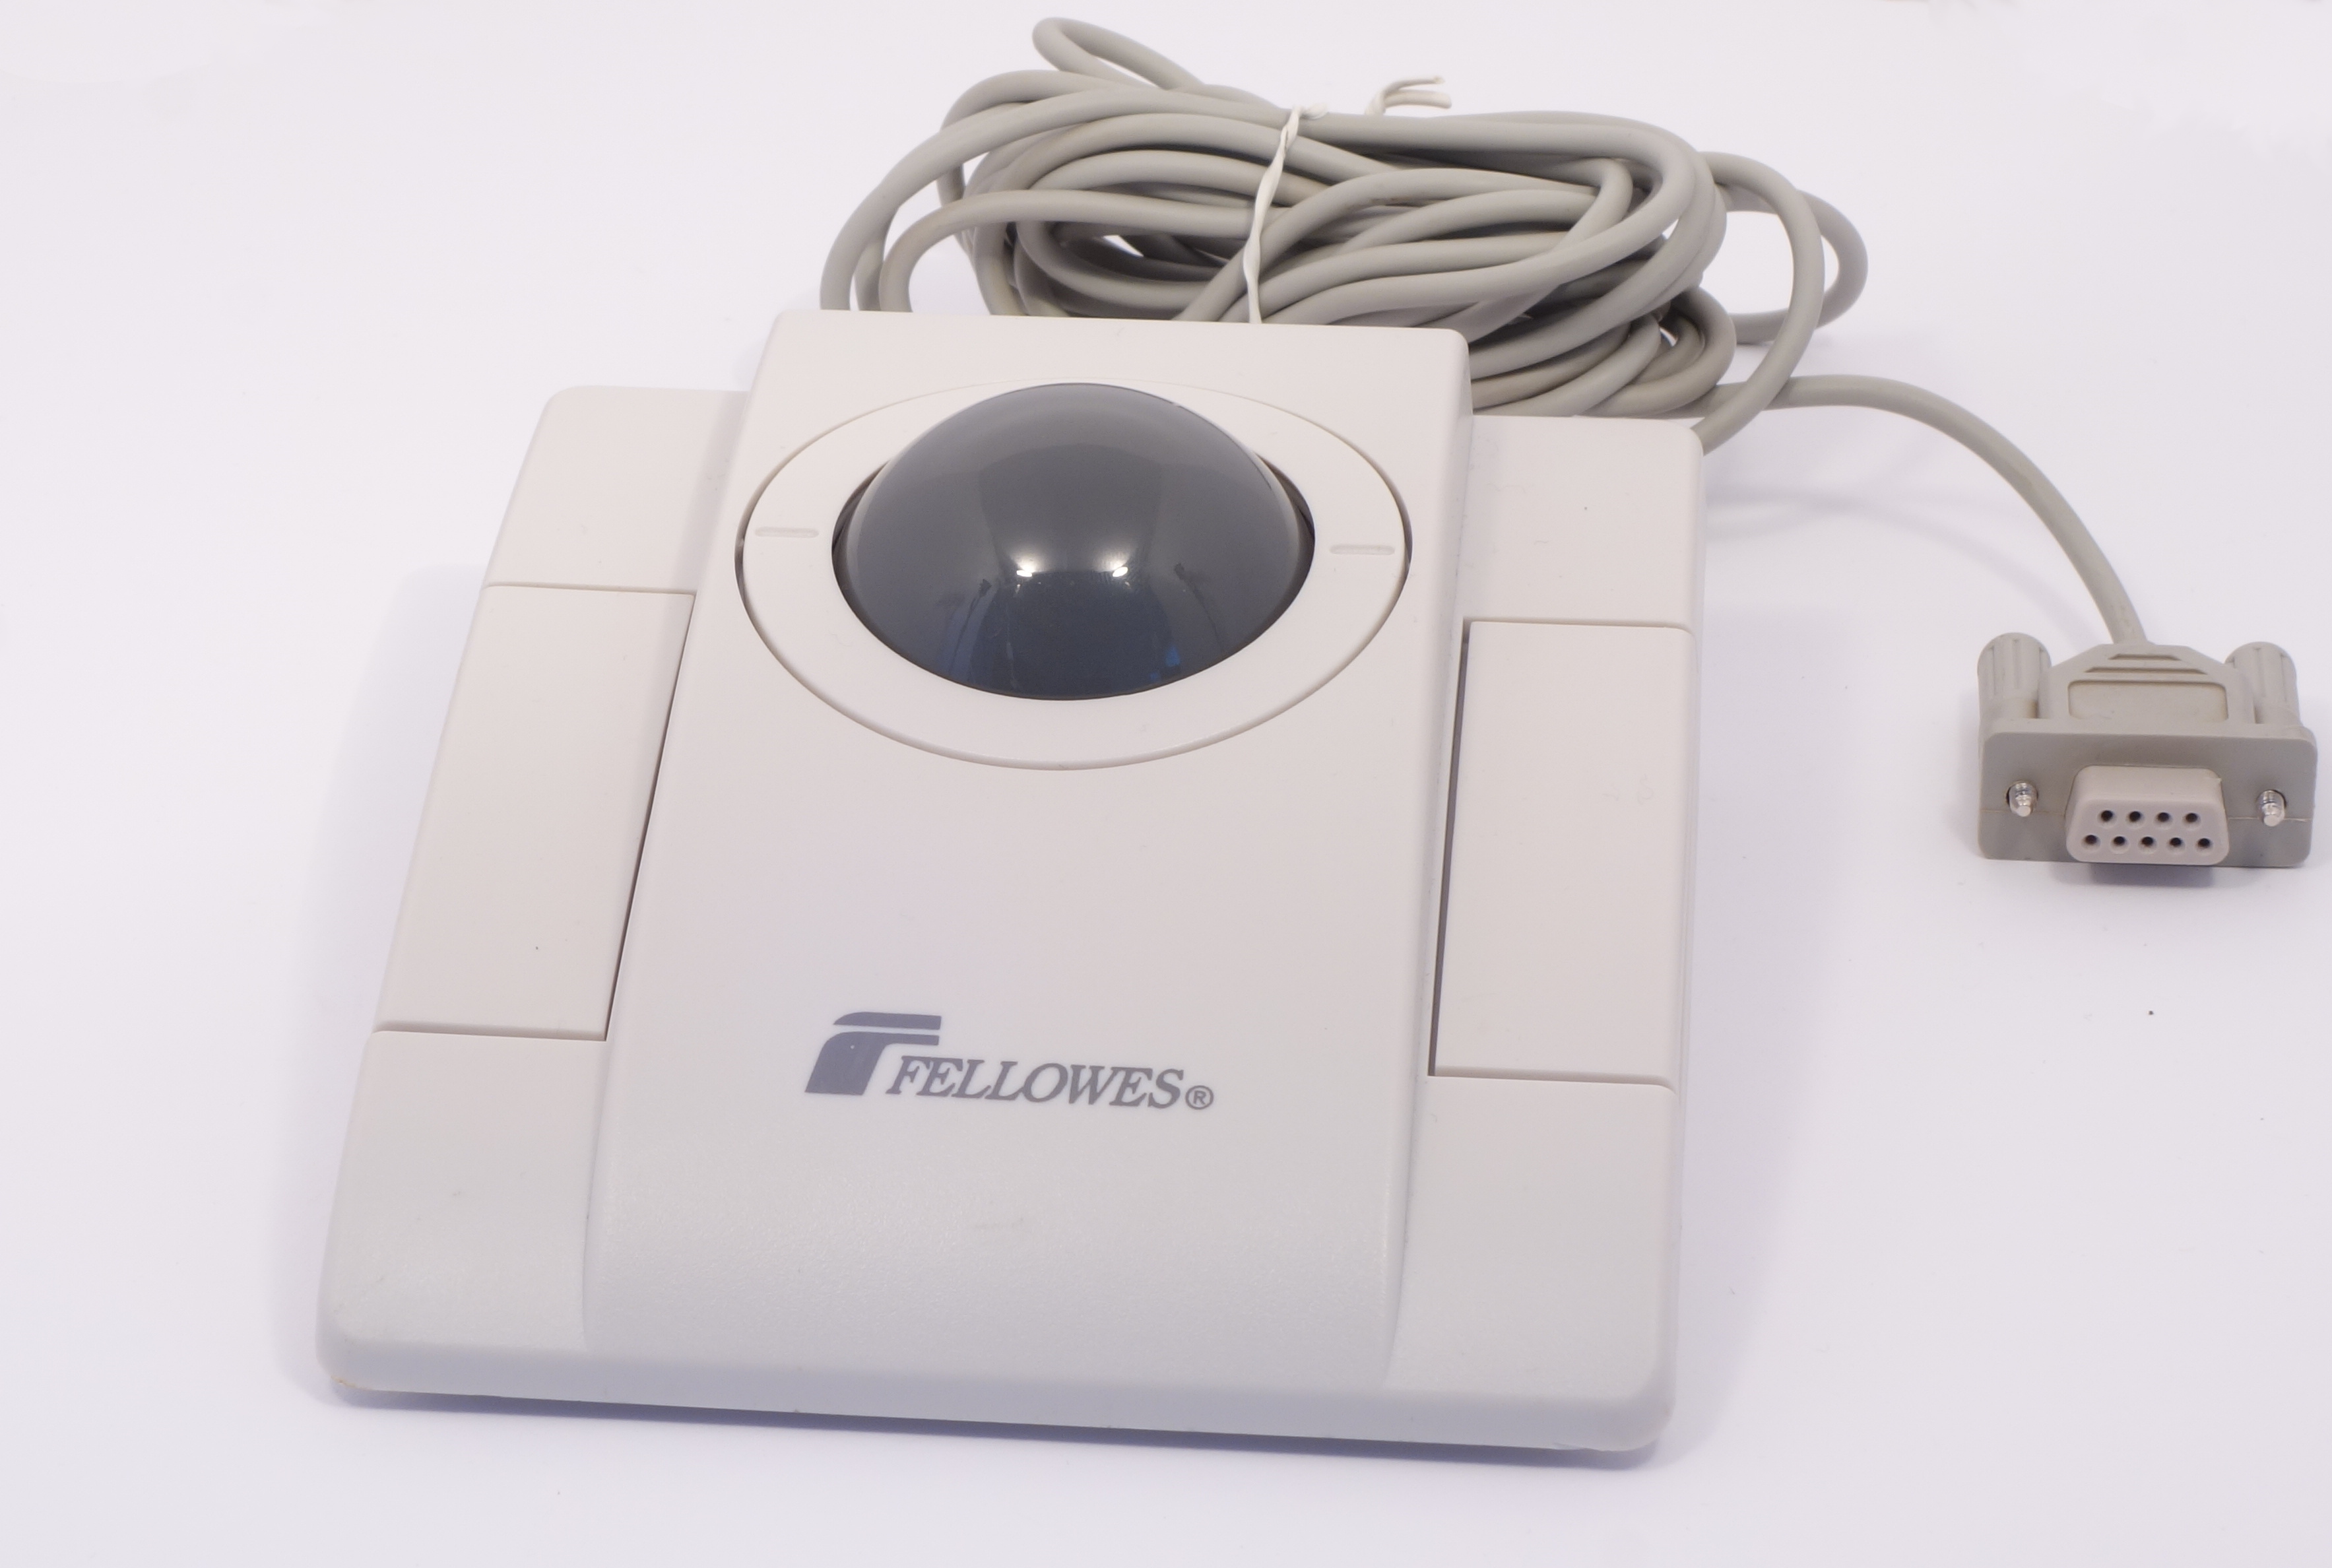
\includegraphics[scale=0.2]{1997_fellowes_trackball/fellowes.jpg}
    \caption{Fellowes Trackball}
    \label{fig:pic}
\end{figure}

Конструктивно трекбол также похож на мышь: вращение шарика приводит в движение пару валиков, соединённых с механическими датчиками, либо, в варианте, появившемся позднее данного, движения шара сканируют размещённые в корпусе оптические датчики. 

\begin{figure}[h]
    \centering
    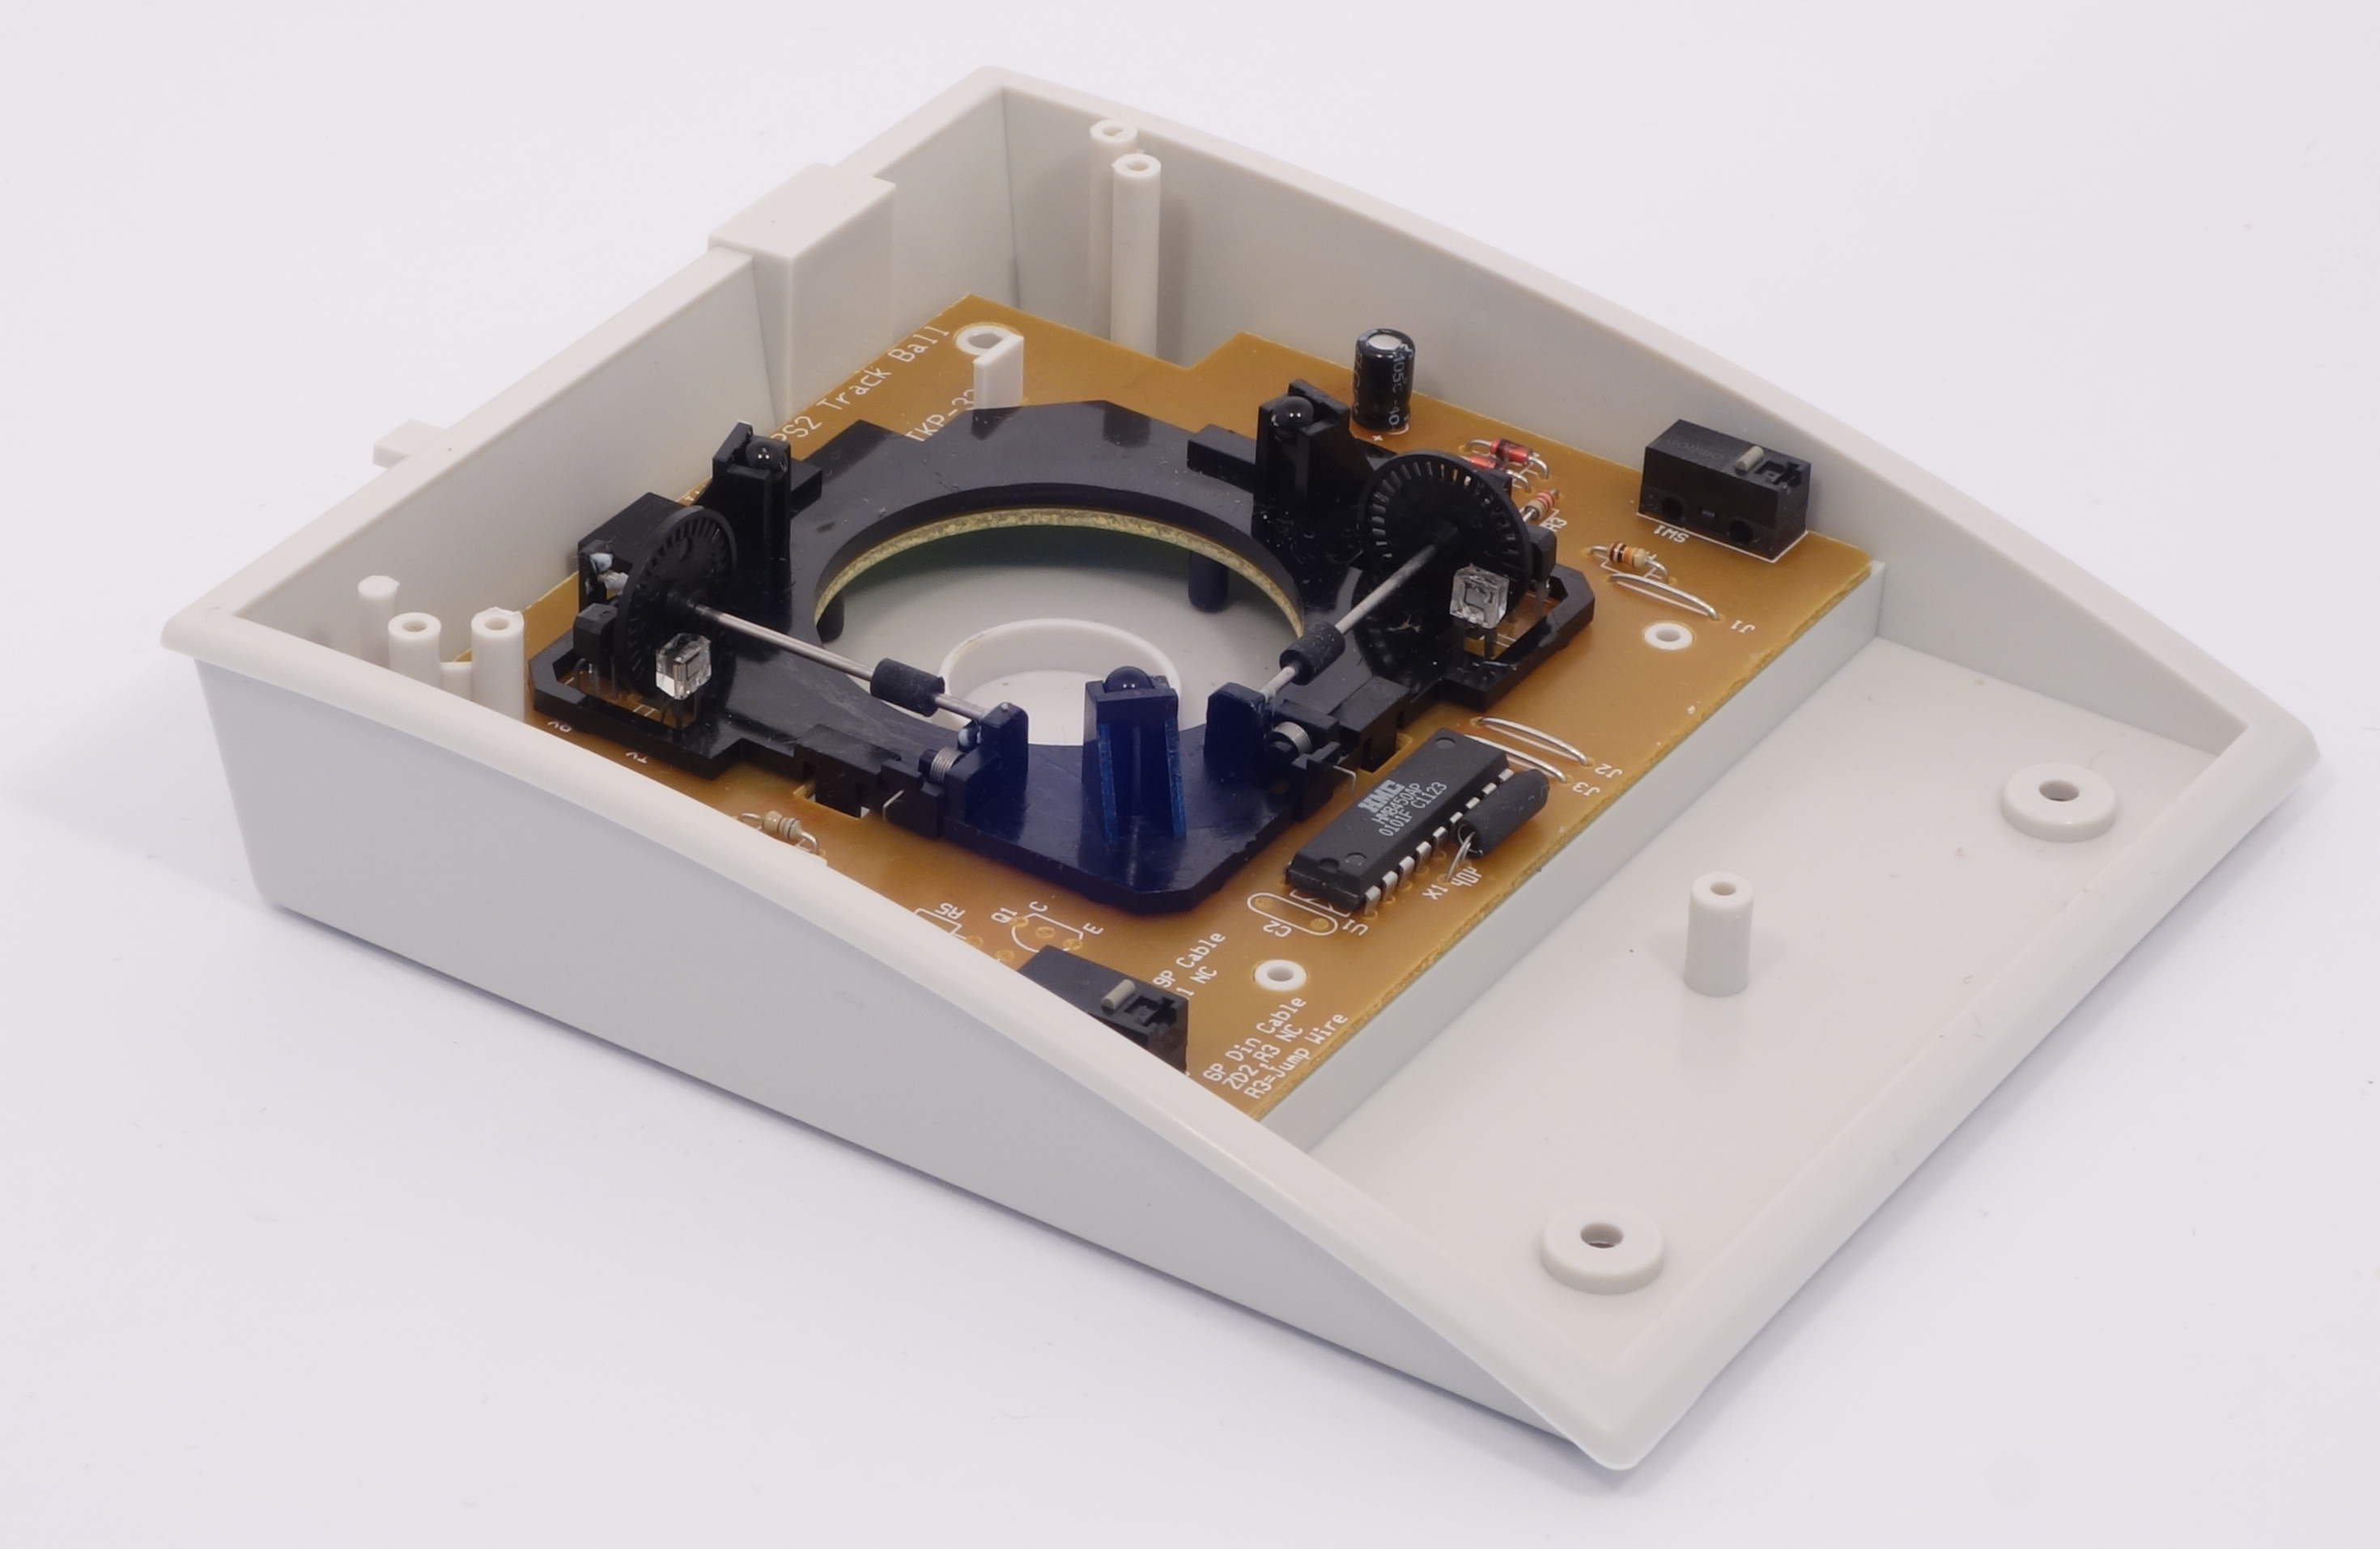
\includegraphics[scale=0.3]{1997_fellowes_trackball/fellowes2.jpg}
    \caption{Fellowes Trackball в разобранном виде}
    \label{fig:inside}
\end{figure}

Протокол обмена данными между трекболом и компьютером, как правило, также полностью соответствует протоколу для мыши. Поэтому с точки зрения компьютера трекбол является стандартным интерфейсным указательным устройством; в отсутствие специальных драйверов он воспринимаются операционной системой компьютера как стандартная мышь и нормально поддерживаются стандартным универсальным драйвером мыши. 

\begin{figure}[h]
    \centering
    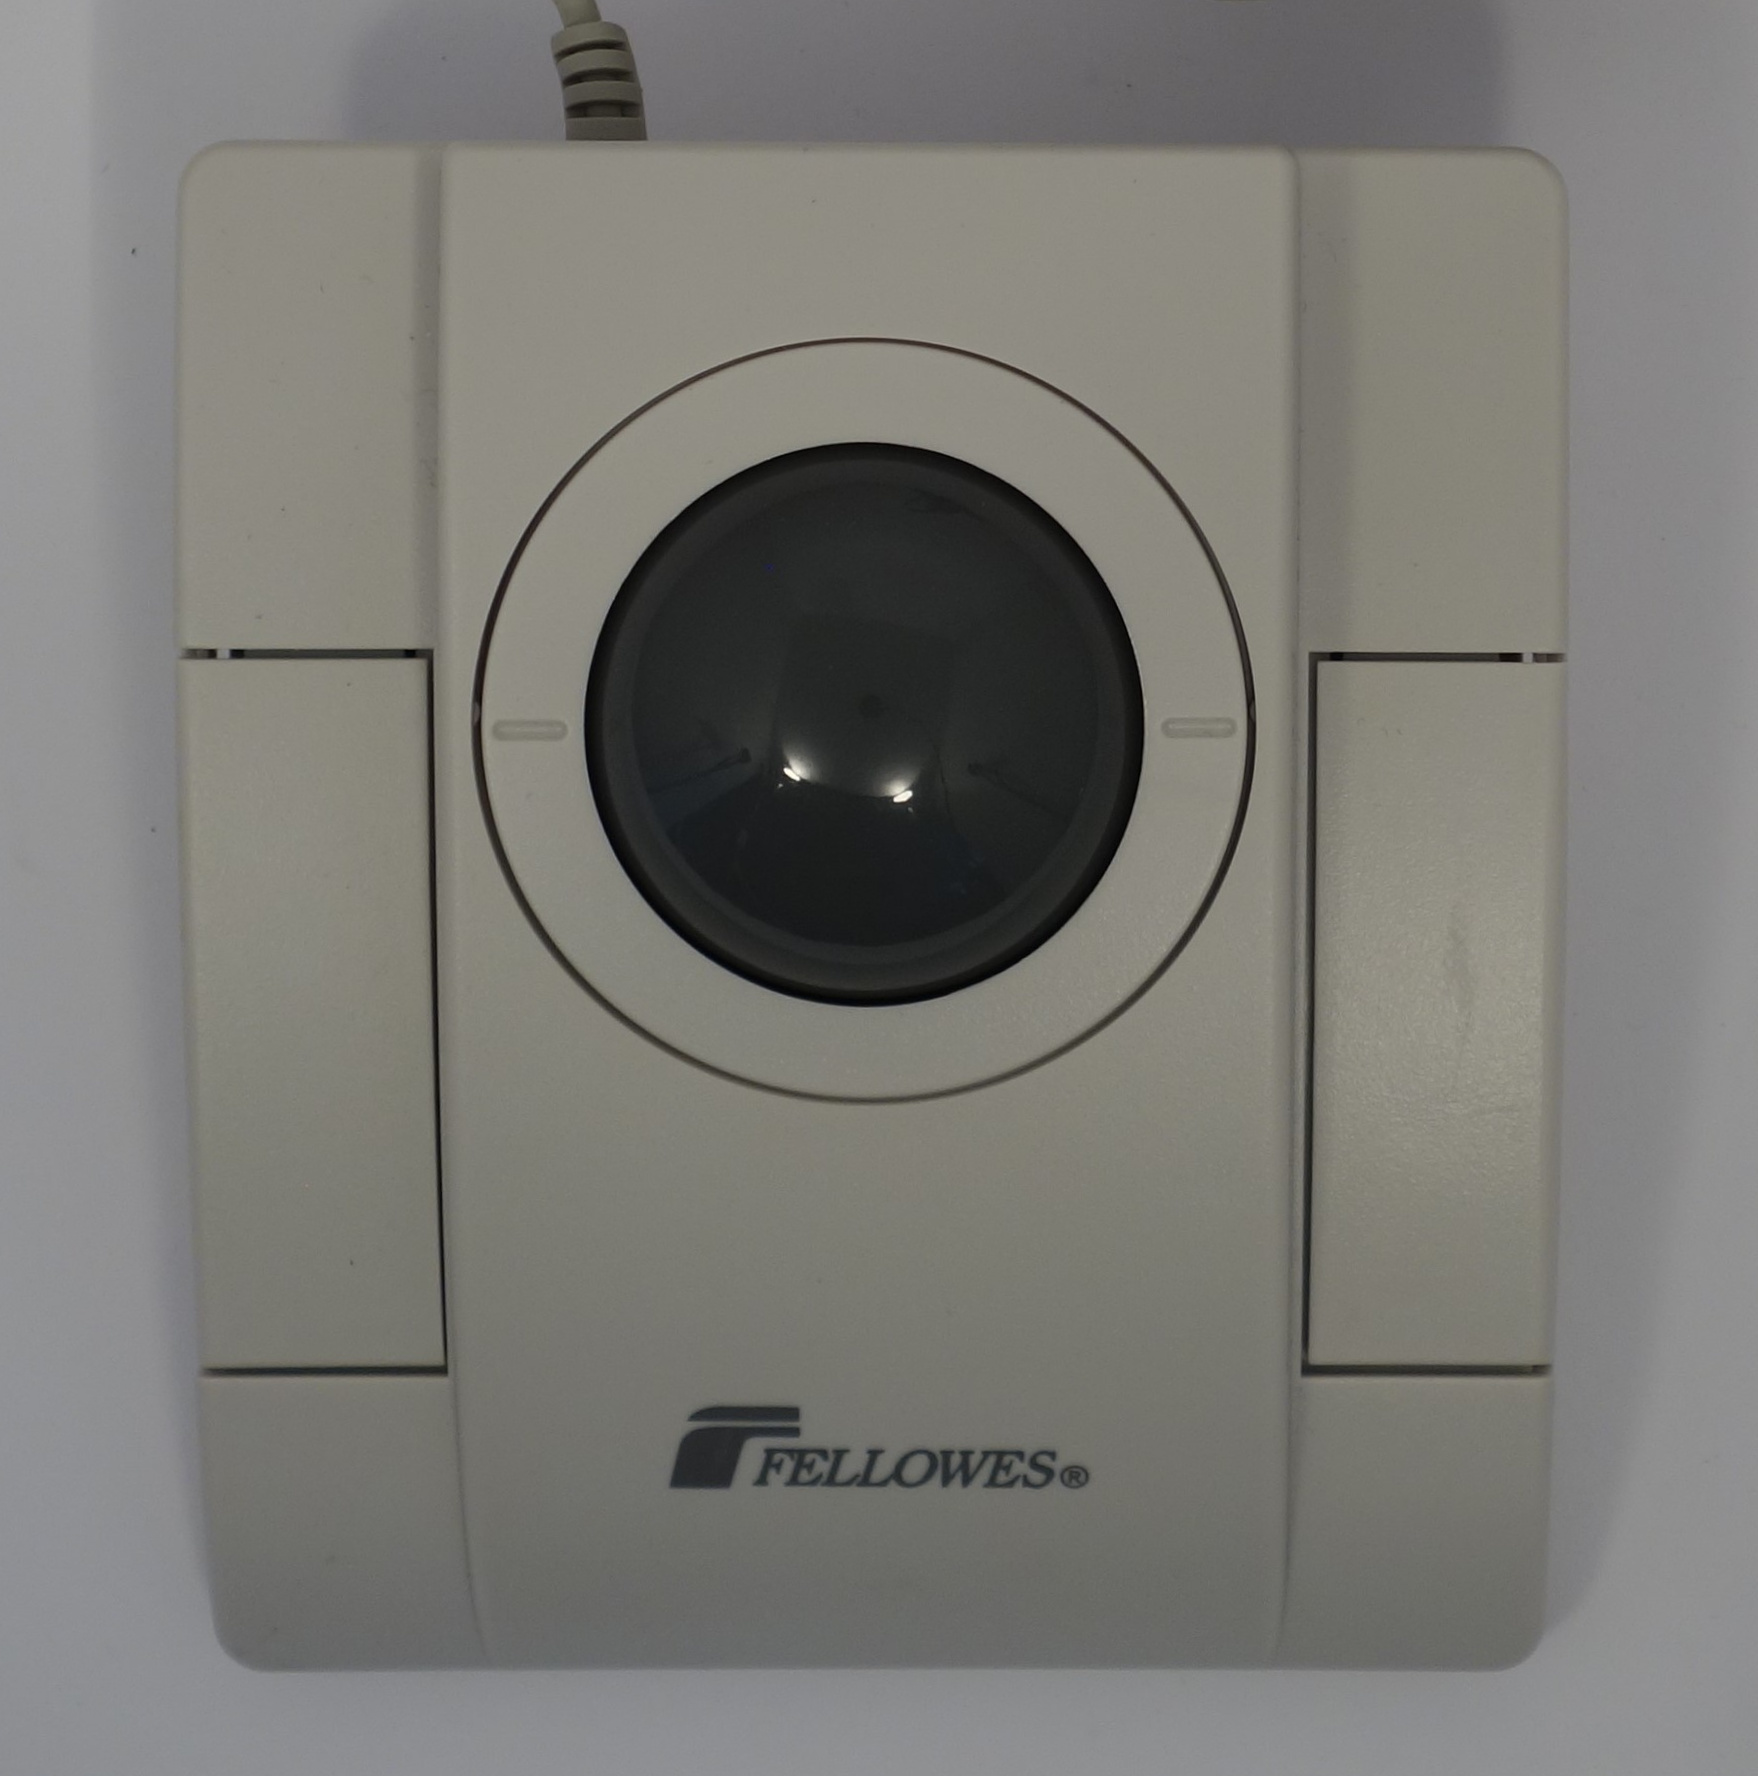
\includegraphics[scale=0.3]{1997_fellowes_trackball/fellowsup.JPG}
    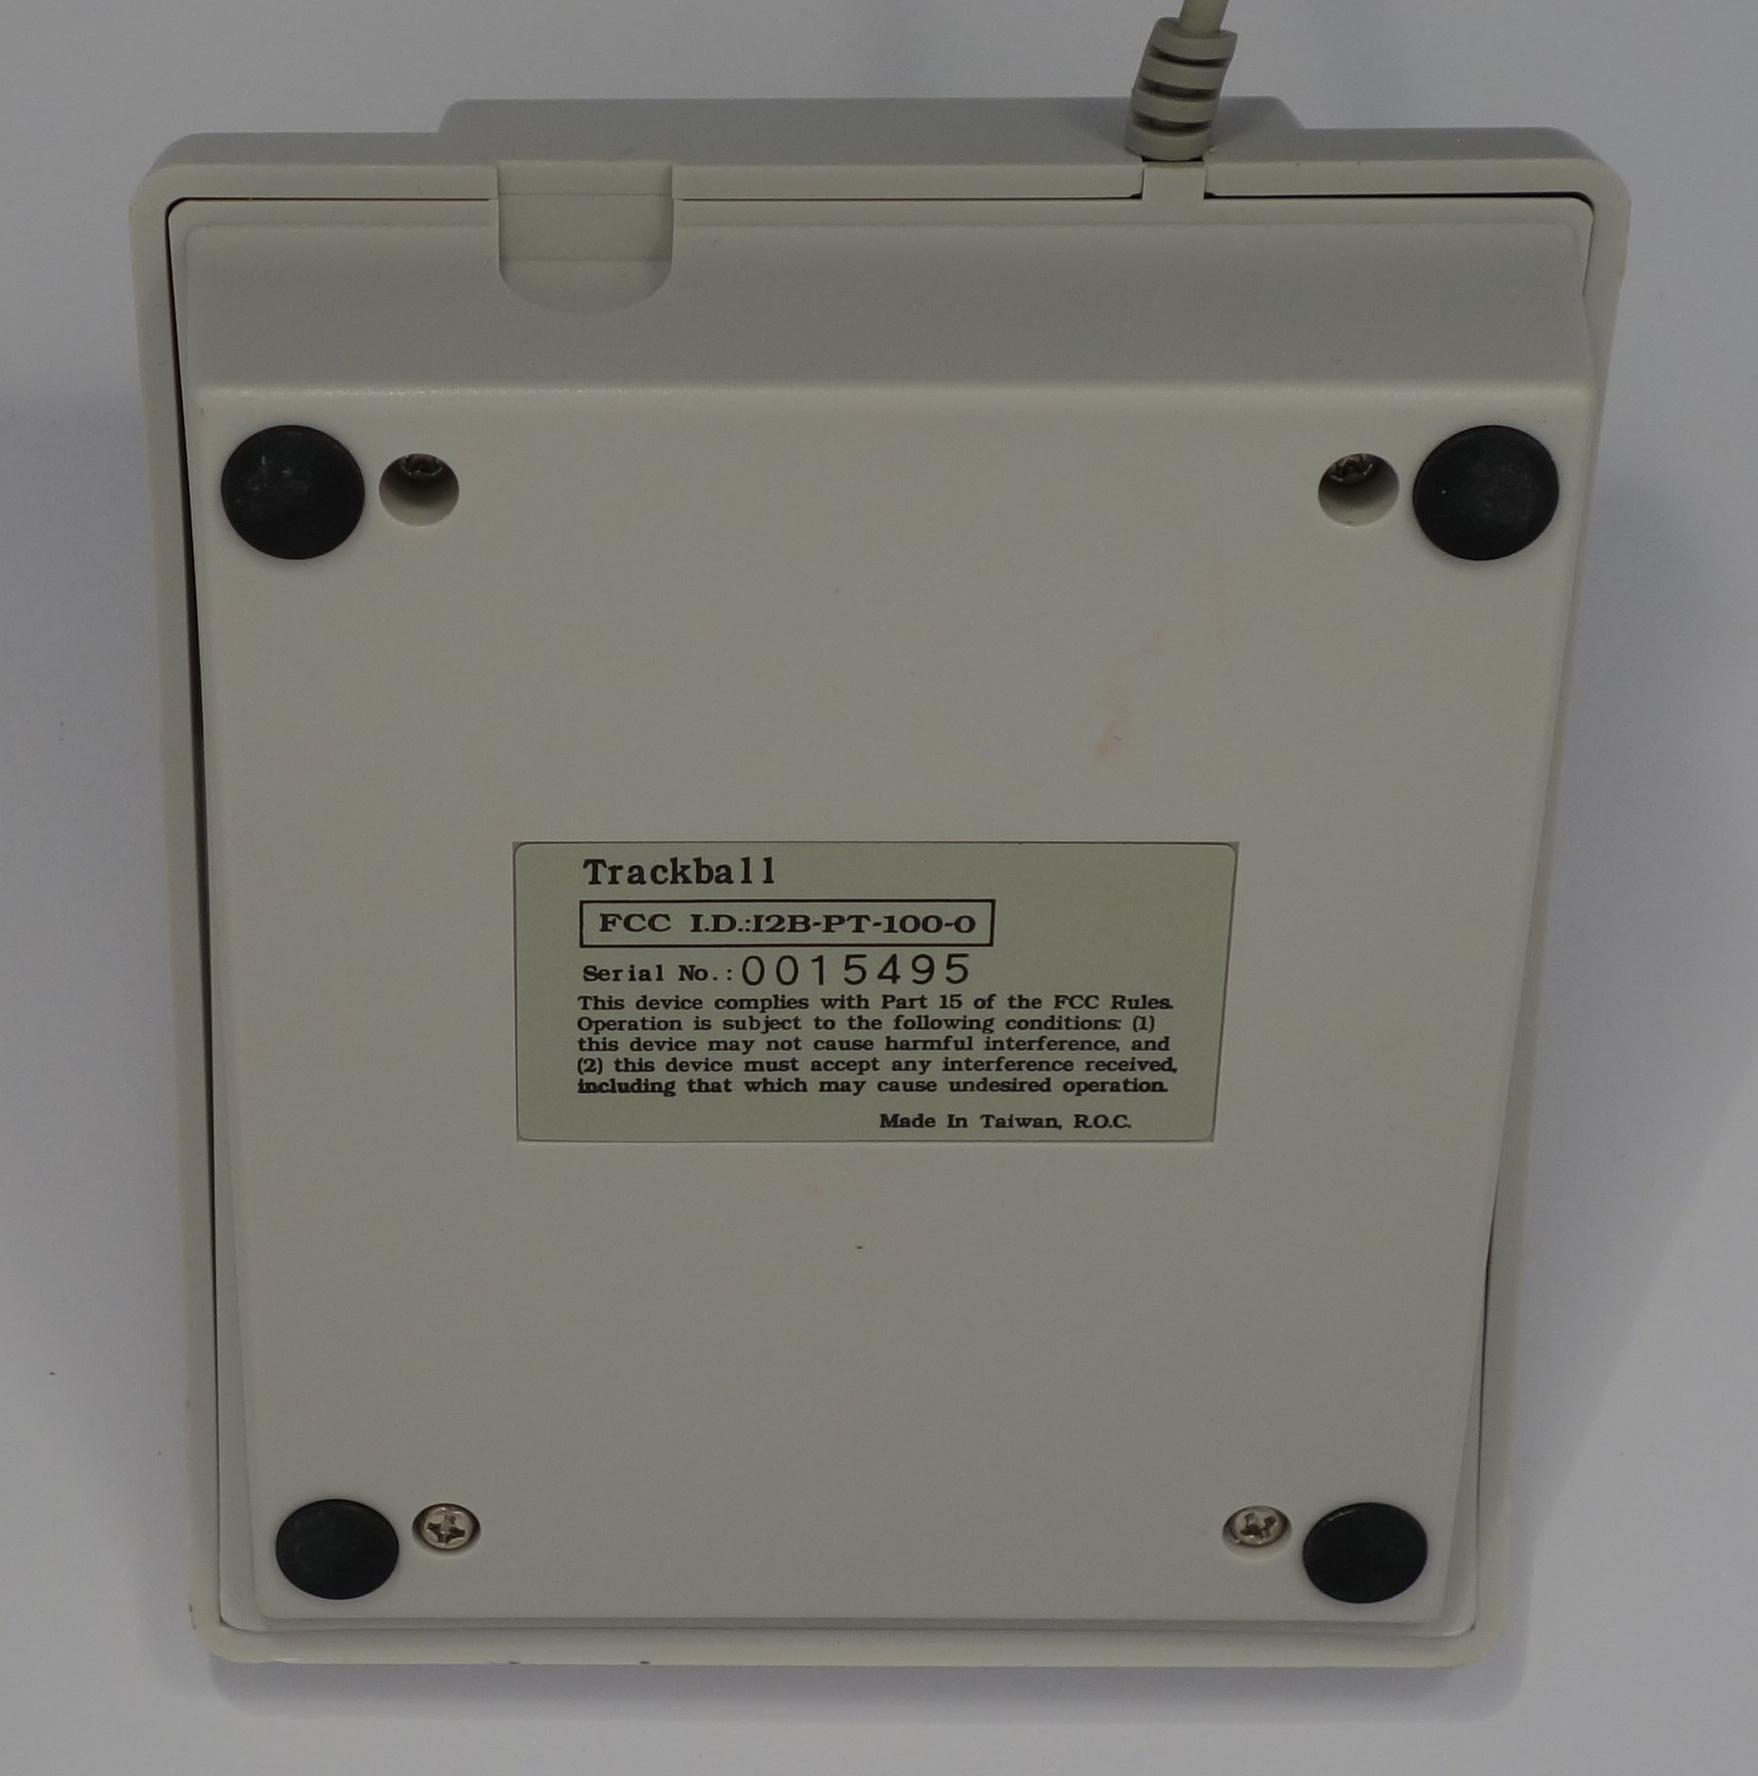
\includegraphics[scale=0.3]{1997_fellowes_trackball/fellowsdown.JPG}
    \caption{Fellowes Trackball, вид сверху и снизу}
    \label{fig:top}
\end{figure}

При работе с трекболом для операций перемещения курсора используется только кисть руки и движения пальцев. Поэтому от пользователя не требуется движений плеча и предплечья, тогда как те же операции с мышью требуют задействования практически всей руки. 
  Поэтому трекбол часто рекомендуется пользователям, испытывающим временные или постоянные проблемы, связанные сплечевым поясом или запястьем.

\begin{figure}[h]
    \centering
    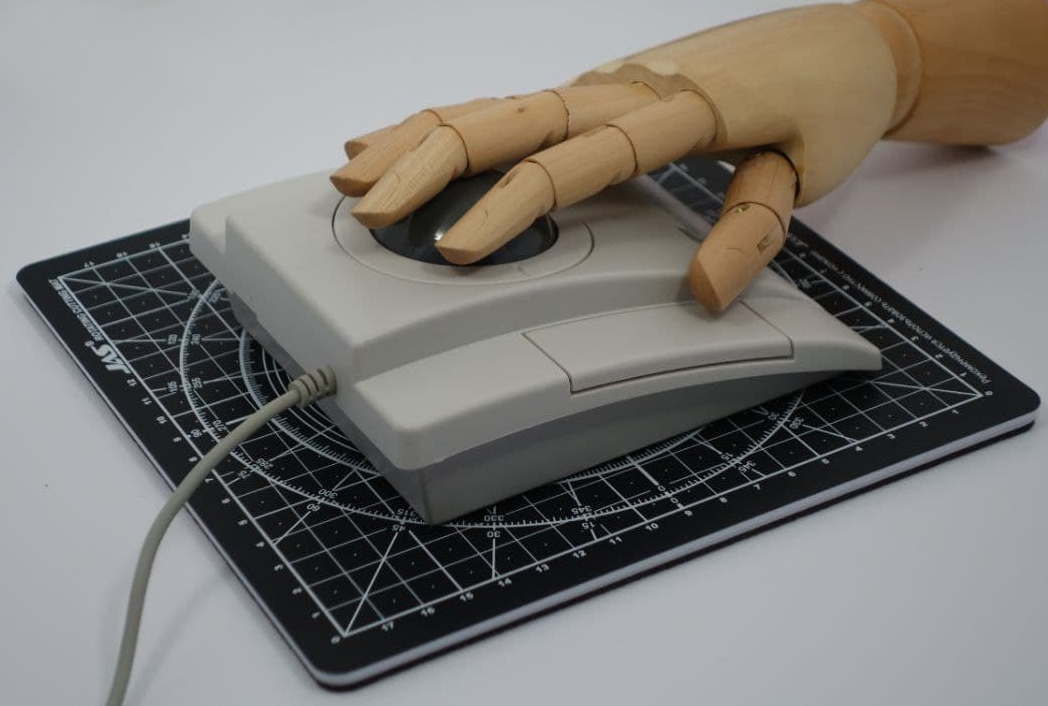
\includegraphics[scale=0.3]{1997_fellowes_trackball/fellowset2.jpg}
    \caption{Fellowes Trackball с моделью руки человека}
    \label{fig:hand}
\end{figure}

В графических приложениях, где позиционирование является основной операцией, использование трекбола, по результатам некоторых исследований, приводит к существенно меньшей усталости и большей точности позиционирования курсора. 

С другой стороны, применение трекбола вместо мыши увеличивает количество движений пальцами, которые вращают шарик, что при активной работе может приводить уже к утомлению пальцев. Также есть сведения, что треболы с шаром, расположенным под большим палцем, способны при длительной и напряженной эксплуатации приводить к проблемам суставов большого пальца.


%\begin{figure}[h]
%    \centering
%    
%    \caption{Fellowes Trackball вид снизу}
%    \label{fig:bottom}
%\end{figure}

\begin{figure}[h]
    \centering
    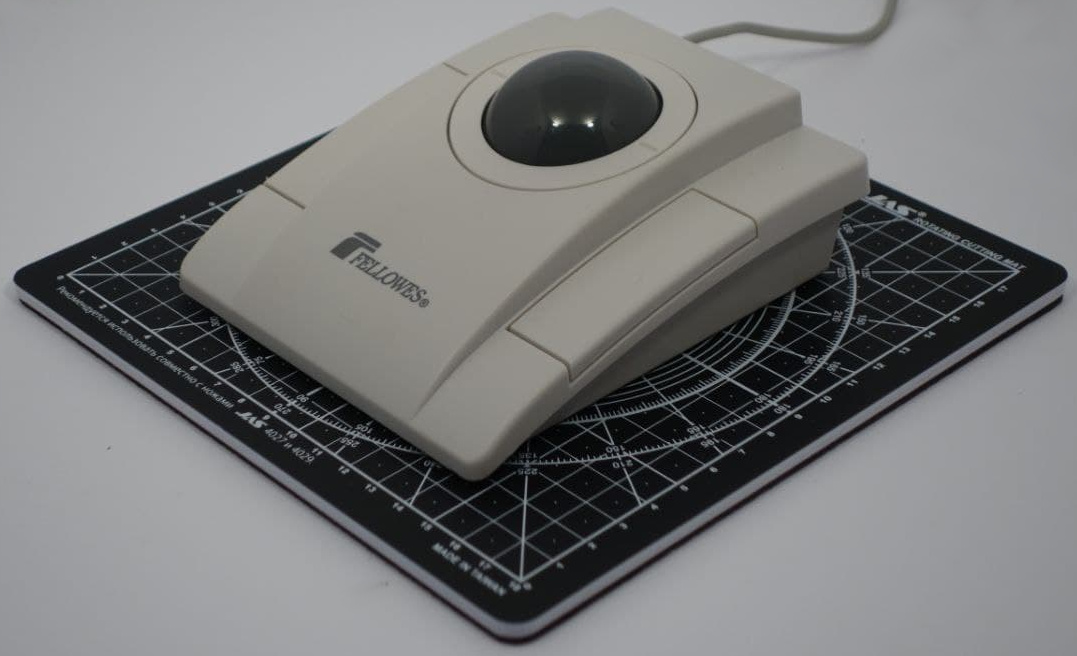
\includegraphics[scale=0.25]{1997_fellowes_trackball/fellowsset.jpg}
    \caption{Fellowes Trackball на размерном коврике с шагом сетки 1~см}
    \label{fig:size}
\end{figure}

Трекбол не требует пространства на рабочем месте, превышающего собственные размеры, его даже можно жёстко закрепить (в том числе на негоризонтальной поверхности), гарантировав, что он случайно не переместится, не упадёт с рабочего места. В условиях ограниченного пространства или необходимости работать в неудобных положениях это может быть решающим аргументом.

Производитель трекбола в рекламных материалах делал упор на высококачественные кнопки большой площади, а также симметричный дизайн, одинаково удобный как для левой, так и для правой руки. В плане совместимости заявлена поддержка ОС Windows начиная с версии 3.1.

